\documentclass{article}

\usepackage{dibrisunige-report}

% Encodings
\usepackage{amsmath,amssymb,gensymb,textcomp}

% Better tables
\usepackage{array,multicol,multirow,siunitx,tabularx}

% Better enum
\usepackage{enumitem}

% Graphics
\usepackage{caption,float}
\usepackage[export]{adjustbox}

\ocoursename{Virtual Reality for Robotics - code 104737 - a.y. 2025/2026}
\oreporttype{Project Report}
\otitle{Few-Shot Gaussian Splatting with Diffusion-Based Data Augmentation}
\oadvisor{Prof. Fabio Solari, Prof. Manuela Chessa}
\reportlayout%

\title{Few-Shot Gaussian Splatting with Diffusion-Based Data Augmentation}
\author{Mohamed Eyad}
\date{\today}

\begin{document}

\coverpage%

\tableofcontents
\newpage

\begin{abstract}
\noindent
Diffusion models can invent photographs that look convincing, which suggests an
obvious remedy when a 3D scene has been captured from too few viewpoints:
generate more views. This report tests that idea on 166 Gaussian-splatting
training runs and finds that it is conditionally false. The same augmentation
that improves a five-view reconstruction by +0.285\,dB degrades a twenty-view
one by -0.618\,dB. Ordering three augmentation strategies by how much
\emph{camera pose} they invent orders them exactly by how much damage they do,
and four controls exclude image quality, hallucinated content, warping
artefacts and mere view repetition as explanations. A synthetic view supplies
coverage and inconsistency together; only the value of coverage decays as real
photographs accumulate.
\end{abstract}

\section{Gaussian splatting when photographs are scarce}

3D Gaussian Splatting~\cite{kerbl3Dgaussians} represents a scene as a set of
anisotropic 3D Gaussians, each carrying a position, covariance, opacity and
view-dependent colour, and rasterises them differentiably so that the primitives
are fitted directly to the training photographs. Given a dense capture it is
both fast and accurate. Given a sparse one it is not: with few views the
photometric objective is badly under-determined, and the optimiser is free to
place primitives that explain the training images while producing floaters and
smeared geometry anywhere the cameras did not look.

The scale of that penalty is the first thing to establish, because every later
number is measured against it. Table~\ref{tab:floors} reports held-out quality
for subsets of 5, 10 and 20 real photographs of the Tanks~\&
Temples~\cite{knapitsch2017tanks} \texttt{truck} scene, against a full-data
ceiling trained on all 219.

\begin{table}[htbp]
  \centering
  \caption{Held-out quality against the number of real training views, three
  seeds per row except the ceiling, which is a single deterministic run. Time
  and primitive count are the per-run cost on an RTX 3050 Ti (4\,GB).}
  \label{tab:floors}
  \begin{tabular}{lccccc}
    \toprule
    \textbf{Real views} & \textbf{PSNR} & \textbf{SSIM} & \textbf{LPIPS}
    & \textbf{Train (s)} & \textbf{Gaussians} \\
    \midrule
    5 & 15.20 $\pm$ 0.33 & 0.538 & 0.410 & 232 & 398k \\
    10 & 17.11 $\pm$ 0.39 & 0.658 & 0.302 & 371 & 494k \\
    20 & 19.74 $\pm$ 0.33 & 0.784 & 0.203 & 305 & 661k \\
    \midrule
    219 (all) & 25.23 & 0.907 & 0.123 & --- & 1033k \\
    \bottomrule
  \end{tabular}
\end{table}

Five views reach 15.20\,dB against a 25.23\,dB ceiling. The marginal
value of a real photograph falls by an order of magnitude across the range:
+0.382\,dB each between five and ten views, +0.028\,dB each
beyond twenty. That decay is what makes synthetic coverage plausible in the
first place, and, as Section~\ref{sec:discussion} argues, it is also why the
idea eventually fails. Figure~\ref{fig:scaling} shows both halves of that
picture on one axis.

\begin{figure}[htbp]
  \centering
  
\includegraphics[width=1.0\textwidth]{figures/scaling.png}
  \caption{Left: held-out quality against the number of real training views, with the full-data ceiling marked. Right: the best and worst synthetic effects on the same axis. Five more real photographs are worth several times the best synthetic condition measured anywhere here.}
  \label{fig:scaling}
\end{figure}


\section{Three diffusion augmentation strategies}

All synthetic images come from Stable Diffusion~1.5
inpainting~\cite{rombach2022ldm}. The three strategies differ in one
respect only --- how much new \emph{camera pose} they invent --- which is what
makes them a usable experimental axis rather than three unrelated tricks.
Figure~\ref{fig:training} shows what each one actually feeds the optimiser.

\begin{description}[leftmargin=1.4em,style=nextline]
  \item[Inpainting.] A mask is placed over part of a real training photograph
  and the region is regenerated. The camera pose is exactly that of the real
  view, and the pose is reused unchanged. No new viewpoint is created.
  \item[Outpainting.] The real image is padded and the diffusion model
  fabricates the border. The camera centre and orientation are unchanged, but
  the effective field of view is widened, so the synthetic image covers scene
  the original frame never recorded.
  \item[Pose-guided synthesis.] A monocular depth map~\cite{yang2024depthanythingv2}
  is estimated for a real view, the image is warped to a genuinely new camera
  interpolated between two real ones, and the disocclusion holes are filled by
  diffusion. This is the only strategy that supplies a viewpoint that does not
  exist in the capture.
\end{description}

\begin{figure}[htbp]
  \centering
  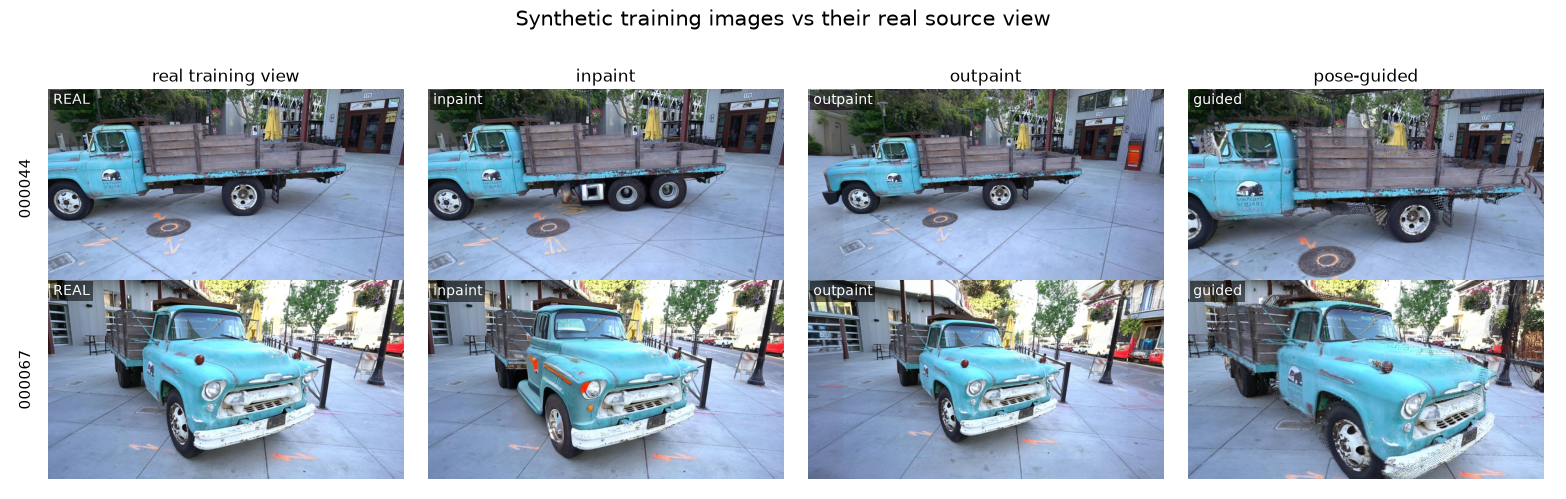
\includegraphics[width=1.0\textwidth]{figures/panel_training_data.png}
  \caption{Synthetic training images beside the real view each derives from. Inpainting has given the truck a second rear axle; outpainting fabricates scene beyond the original frame; pose-guided renders a genuinely different viewpoint, with roughly 10\% of its pixels invented.}
  \label{fig:training}
\end{figure}

Poses for real views come from COLMAP~\cite{schoenberger2016sfm}. Synthetic
views inherit the pose of the real image they derive from, exactly for
inpainting and outpainting, and by interpolation for pose-guided synthesis.

\section{The experiment grid and protocol}

Three subset sizes ($k = 5, 10, 20$) are crossed with three strategies and
five synthetic ratios ($0, 25, 50, 100, 200\%$ of $k$), each repeated over
three seeds --- 166 training runs in total for the primary scene.

Three details carry most of the study's reliability.

\begin{enumerate}[leftmargin=1.6em]
  \item \textbf{A frozen held-out set.} Thirty-two real photographs are
  reserved once and never trained on by any run, so every number in this report
  is comparable across every condition. Synthetic images are only ever added to
  \emph{training}.
  \item \textbf{Pairing within seed.} Each augmented run is compared against
  the zero-synthetic baseline built from \emph{the same seed's} subset, so the
  difficulty of a particular draw of $k$ photographs cancels rather than
  appearing as an effect.
  \item \textbf{A measured noise floor.} Repeating an identical configuration
  gives a run-to-run standard deviation of 0.039\,dB. Any effect smaller
  than roughly $\sqrt{2}\times$ that is indistinguishable from noise, and is
  reported as such. Three seeds support a consistency check --- marked * where
  $|\text{mean}|$ exceeds the between-seed spread --- not a significance test.
\end{enumerate}

Quality is reported as PSNR and SSIM, the two metrics the brief
specifies, with LPIPS~\cite{zhang2018lpips} added because neither of the
first two is perceptual. SSIM follows Wang et al.~\cite{wang2004ssim}.

\section{Results}

Table~\ref{tab:grid} is the full grid: the paired change in PSNR for every
strategy, ratio and subset size, and Figure~\ref{fig:paired} plots the same
quantities against the measured noise floor.

\begin{table}[htbp]
  \centering
  \caption{Paired $\Delta$PSNR against the same seed's zero-synthetic
  baseline. Rows are grouped by strategy; within each strategy the three lines
  are $k = 5$, $10$ and $20$. Columns are the synthetic ratio. * marks a mean
  exceeding its between-seed standard deviation.}
  \label{tab:grid}
  \begin{tabular}{lcccc}
    \toprule
    \textbf{Strategy} & \textbf{25\%} & \textbf{50\%} & \textbf{100\%}
    & \textbf{200\%} \\
    \midrule
    Inpainting & -0.039 & -0.142\,* & -0.166\,* & +0.029 \\
     & +0.014 & -0.142\,* & -0.213\,* & -0.141 \\
     & -0.032 & -0.073\,* & -0.161\,* & -0.102\,* \\
    \addlinespace
    Outpainting & +0.140\,* & +0.140\,* & +0.182\,* & +0.285\,* \\
     & +0.172\,* & +0.013 & -0.423\,* & -0.003 \\
     & -0.283\,* & -0.542\,* & -0.983\,* & -0.618\,* \\
    \addlinespace
    Pose-guided & -0.309\,* & -0.375\,* & -0.719\,* & -1.013\,* \\
     & -0.451\,* & -0.855\,* & -1.404\,* & -1.451\,* \\
     & -1.017\,* & -1.528\,* & -1.729\,* & -1.884\,* \\
    \addlinespace
    \bottomrule
  \end{tabular}
\end{table}

\begin{figure}[htbp]
  \centering
  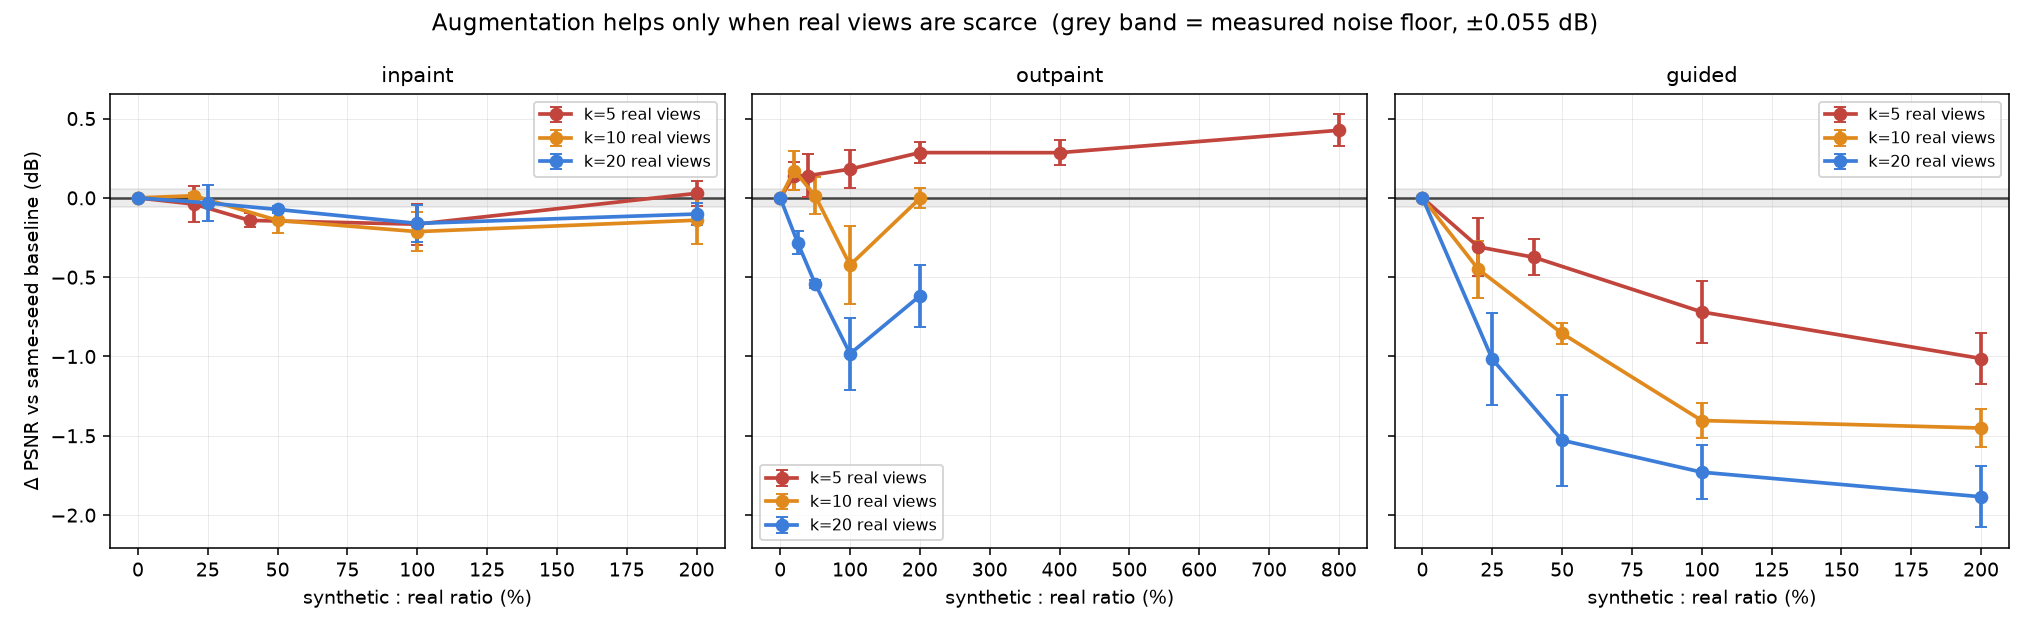
\includegraphics[width=1.0\textwidth]{figures/curves_paired.png}
  \caption{Paired change in PSNR against each seed's own zero-synthetic baseline, one line per subset size. Error bars are the standard deviation across three seeds; the grey band is the measured noise floor. Inpainting is flat, outpainting crosses over, pose-guided is harmful everywhere.}
  \label{fig:paired}
\end{figure}

\subsection{The crossover}

Outpainting is positive at every ratio at five real views and negative at every
ratio at twenty: +0.285 $\pm$ 0.069\,*\,dB at $k = 5$ against -0.618 $\pm$ 0.195\,*\,dB at $k = 20$. The
sign of the effect depends on how much real data is already present, not on the
method or on the ratio.

The other two strategies bracket the explanation. Inpainting, which reuses the
camera pose exactly, is flat everywhere --- between -0.213 and +0.029\,dB
--- despite producing convincing images. Pose-guided synthesis, which invents a
fully novel viewpoint, is harmful at every subset size and worsens as $k$ grows,
reaching -1.884\,dB. Ordering the three by invented camera pose orders them
by damage. Figure~\ref{fig:crossover} shows the same treatment helping and
harming side by side, and Figure~\ref{fig:strategies} gives held-out
renderings for each condition.

\begin{figure}[htbp]
  \centering
  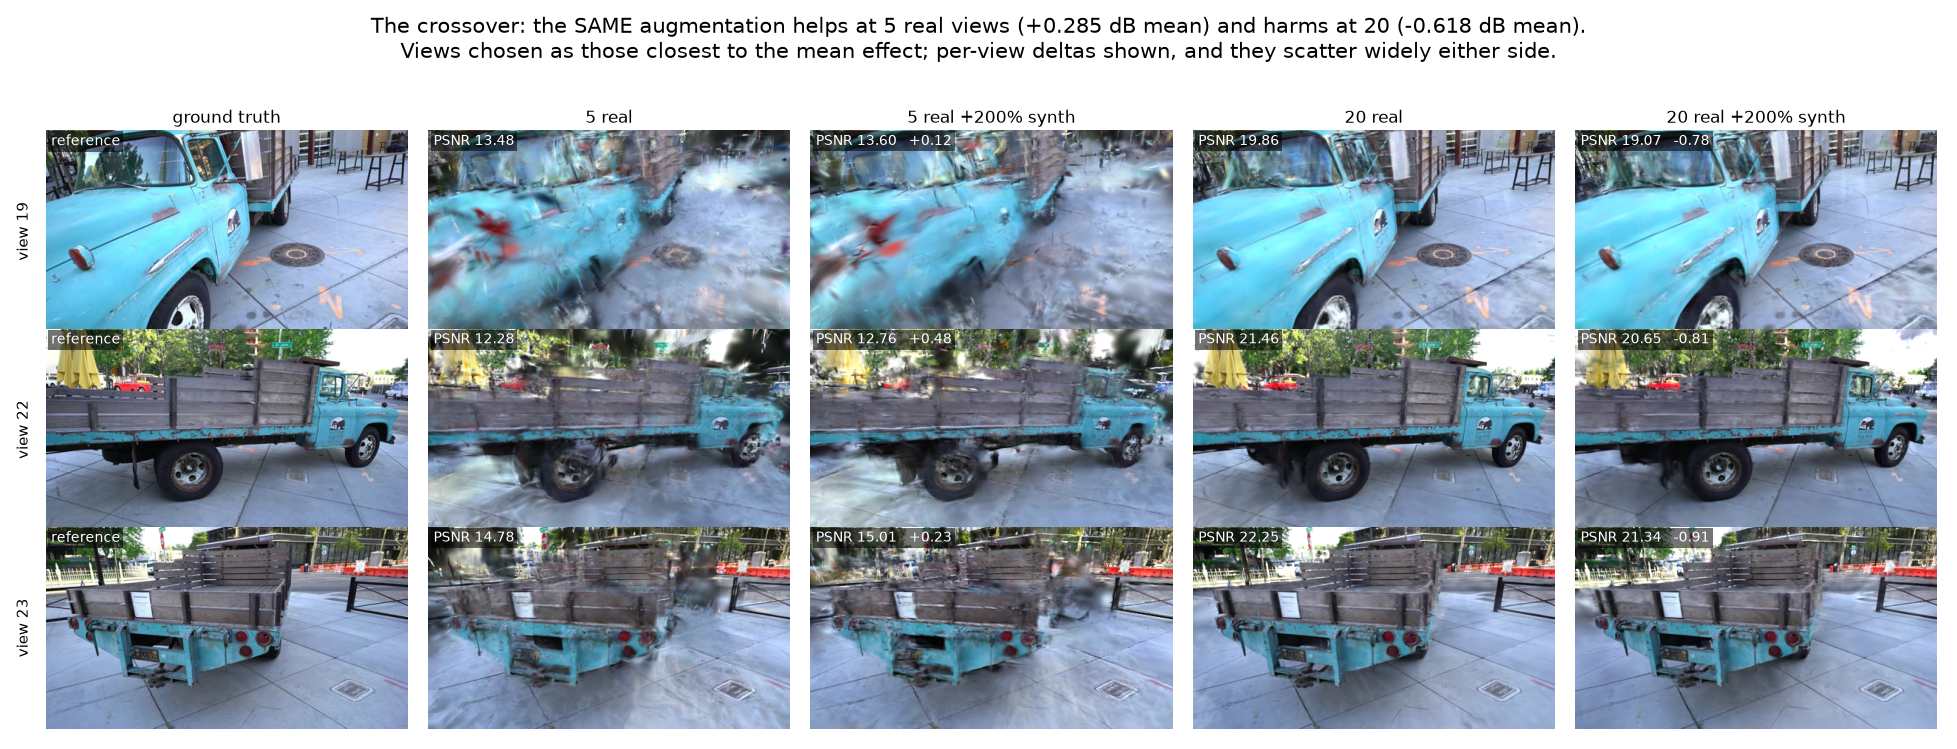
\includegraphics[width=1.0\textwidth]{figures/panel_crossover.png}
  \caption{The crossover made visible: the same 200\% outpainting treatment at five real views and at twenty. Views are those whose per-view delta sits closest to the mean effect.}
  \label{fig:crossover}
\end{figure}

\begin{figure}[htbp]
  \centering
  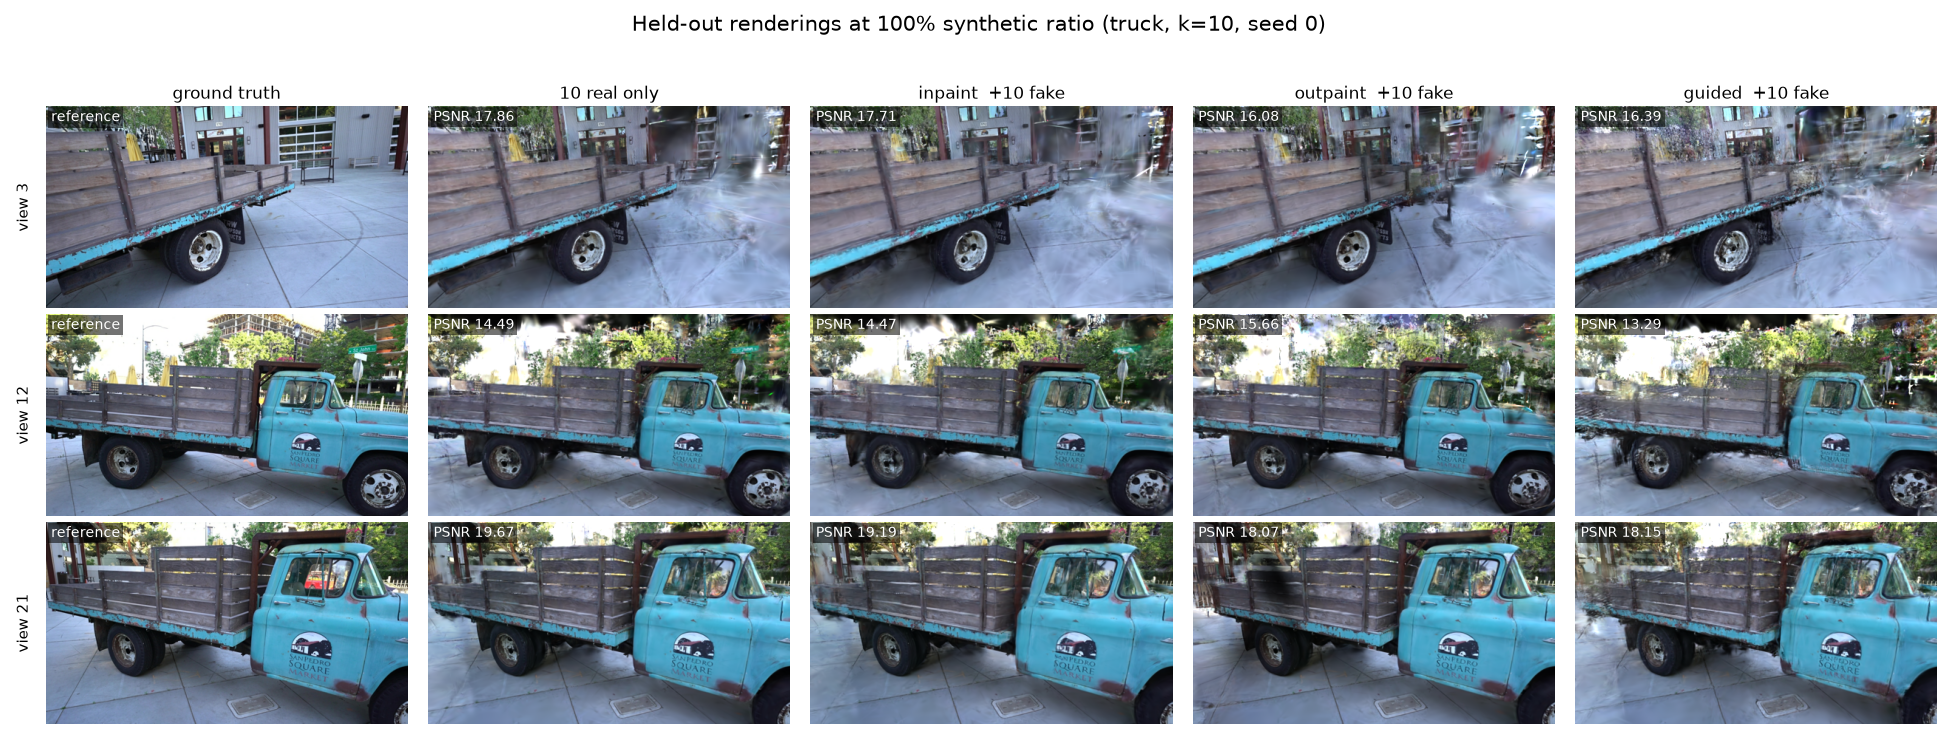
\includegraphics[width=1.0\textwidth]{figures/panel_strategies.png}
  \caption{Held-out renderings for each condition at the 100\% synthetic ratio. Degradation appears as smearing and semi-transparent floaters, most severely under pose-guided synthesis.}
  \label{fig:strategies}
\end{figure}

\subsection{Both required metrics}

Table~\ref{tab:metrics} reports PSNR and SSIM together at the 200\% ratio.

\begin{table}[htbp]
  \centering
  \caption{Both specified metrics at the 200\% ratio, three seeds, paired
  within seed. Note the disagreement at $k = 5$.}
  \label{tab:metrics}
  \begin{tabular}{lcccccc}
    \toprule
    & \multicolumn{2}{c}{$k = 5$} & \multicolumn{2}{c}{$k = 10$}
    & \multicolumn{2}{c}{$k = 20$} \\
    \cmidrule(lr){2-3} \cmidrule(lr){4-5} \cmidrule(lr){6-7}
    \textbf{Strategy} & $\Delta$PSNR & $\Delta$SSIM & $\Delta$PSNR
    & $\Delta$SSIM & $\Delta$PSNR & $\Delta$SSIM \\
    \midrule
    Inpainting & +0.029 & +0.0032\,* & -0.141 & -0.0109\,* & -0.102\,* & -0.0096\,* \\
    Outpainting & +0.285\,* & -0.0054\,* & -0.003 & -0.0227\,* & -0.618\,* & -0.0400\,* \\
    Pose-guided & -1.013\,* & -0.0990\,* & -1.451\,* & -0.1232\,* & -1.884\,* & -0.1180\,* \\
    \bottomrule
  \end{tabular}
\end{table}

The headline gain is \textbf{PSNR-only}. Outpainting at $k = 5$ is worth
+0.285\,dB but -0.0054 SSIM, consistently across all three seeds. PSNR rewards
the reduction in large errors where synthetic coverage fills an unobserved
region; SSIM penalises the local structural noise the fabricated pixels
introduce. The \emph{ordering} of the three strategies holds on both metrics;
the \emph{sign} of outpainting's benefit at $k = 5$ does not.

\subsection{Controls}

Four controls each remove one candidate explanation. Repeating real images to
the same count instead of generating new ones recovers only part of
outpainting's gain, so the fabricated borders --- not mere repetition --- carry
most of it. Skipping diffusion and leaving the warped holes black costs a
further 2.49\,dB, so the diffusion step repairs rather than causes
pose-guided damage. Swapping the checkpoint for DreamShaper-8 reproduces the
sign change, so the effect is not an artefact of one model. Finally, replacing
outpainted borders with plain white isolates fabrication from framing.

The benefit also reproduces on a second, indoor scene, \texttt{drjohnson}
from Deep Blending~\cite{hedman2018deepblending}: +0.989\,dB at $k = 5$ at the
200\% ratio, larger than on \texttt{truck}. The reversal at $k = 20$ is
\emph{weaker} there and should not be overstated --- negative at the 25, 50 and
100\% ratios but +0.195~$\pm$~0.410\,dB at 200\%, which is indistinguishable
from zero. What transfers between scenes is the benefit at small $k$; the harm at
large $k$ transfers in sign but not reliably in magnitude.

\section{Discussion: when synthetic data helps, and when it hurts}
\label{sec:discussion}

\paragraph{A two-term account.} A synthetic view supplies two things at once:
\emph{coverage} of scene geometry the real views did not record, and
\emph{inconsistency} with them, because the fabricated pixels are not
photographs of anything. Coverage loses value as real views accumulate --- that
is precisely the per-view decay in Table~\ref{tab:floors}, an order of
magnitude across the range. Inconsistency does not decay. A contradictory view
is at least as harmful at twenty real views as at five, and arguably worse,
because it now contradicts a better-determined geometry. Two terms, one
decaying and one roughly constant, are sufficient to produce a sign change, and
that is what the grid shows.

\paragraph{Increasing reliance on synthetic data.} Reliance can be increased
along two axes, and they behave differently. Raising the \emph{ratio} at fixed
$k$ is comparatively benign where the balance is already favourable --- at
$k = 5$ outpainting stays positive from 25\% to 200\% --- and monotonically
damaging where it is not. Lowering the proportion of \emph{real} data at a
fixed ratio is what actually reverses the sign. The practical reading is that
synthetic images are a substitute for photographs only in the regime where
photographs are very scarce, and never a supplement to an adequate capture.

\paragraph{A constraint that does not cross over.} If the harm comes from
invented viewpoints rather than from augmentation as such, then an intervention
that constrains geometry \emph{without} inventing a camera should never
reverse sign. Monocular depth regularisation is that intervention, and it is
prior work rather than a contribution here: Chung et al.~\cite{chung2023depthreg}
propose the same construction --- a dense monocular depth map as a geometry
guide, scale-aligned against sparse COLMAP points. Used as a control, it is
worth +0.259\,dB at $k = 5$ and remains positive at +0.155\,dB at $k = 20$,
where outpainting costs -0.618. Combined with outpainting at $k = 5$ it
reaches +0.714\,dB, the largest improvement measured in this study. Coverage
crosses over; constraint does not.

\paragraph{The result is conditional on early stopping.} Training longer
decays the benefit monotonically: outpainting at $k = 5$ falls from +0.285 to
+0.045 at 15{,}000 iterations and -0.078 at 30{,}000. The unaugmented
baseline is flat from 7{,}000 to 15{,}000 (15.20~$\rightarrow$~15.22\,dB)
and lower by 30{,}000 (15.04\,dB), so 7{,}000 is a fair operating point
rather than a flattering one --- few-shot splatting overfits well before
30{,}000. The depth prior is the exception: at 30{,}000 iterations outpainting
alone is worth -0.078\,dB while the prior still returns +0.208 and the two
together +0.469. Fabricated pixels lose their value to longer training; a
geometric constraint does not.

\section{Conclusions}

\begin{itemize}[leftmargin=1.4em]
  \item Diffusion augmentation is not free coverage. It helps only while real
  views are scarce, and the crossover reproduces on an outdoor object and an
  indoor room.
  \item The mechanism is invented camera pose. Four controls exclude image
  quality, hallucinated hole content, warping artefacts and view repetition.
  \item Constraint beats invention where data is plentiful: a depth prior never
  crosses over and costs no diffusion model.
  \item Scale honestly --- the best synthetic condition measured anywhere is
  worth a small fraction of simply taking five more photographs.
\end{itemize}

\paragraph{Limitations.} Three seeds support a consistency check, not a
significance test. The crossover is bracketed between $k = 5$ and $k = 20$, not
located. Both diffusion checkpoints are SD~1.5-class, the only ones fitting
4\,GB of VRAM; multi-view-consistent generators are the natural next step and
are arguably what pose-guided augmentation is really reaching for. The positive
result is conditional on both the early-stopped operating point and the choice
of metric, as stated above.

\bibliographystyle{plain}
\bibliography{refs}

\end{document}
